%!TEX root = main.tex
\begin{figure*}[t!]
\centering
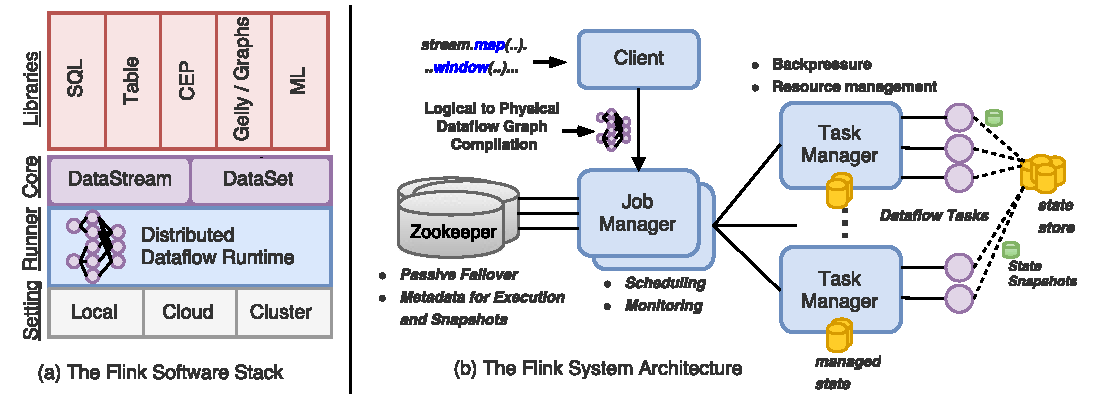
\includegraphics[width=\textwidth]{figures/flinkoverview.pdf}
\caption{An Overview of the Apache Flink System Model and Architecture.} 
\label{fig:flink-overview}
\vspace{-4mm}
\end{figure*}

\section{Preliminaries}
\label{sec:preliminaries}
\subsection{The Apache Flink System}

The Apache Flink system \cite{CUSTOM:web/Flink} is an open-source project that provides a full software stack for programming, compiling and running distributed continuous data processing pipelines (\autoref{fig:flink-overview}(a)). Pipelines can be written as a series of data-centric transformations expressed in a fluid, functional programming API (in Scala, Java or Python) inspired by Flume Java\cite{chambers2010flumejava}, Dryad LINQ\cite{yu2008dryadlinq}, Naiad\cite{murray2013naiad} and the Dataflow Model \cite{akidau2015dataflow}. At the core of the model there are two basic abstract data types, the \emph{DataSet} and \emph{DataStream} representations which target bounded and unbounded datasets respectively. Computation declared using the available higher-level domain-specific libraries such as the SQL and Machine Learning (ML) packages, in fact, translates into a logical pipeline using these core representations. A major distinctive trait of the Flink programming model compared to state of the art is the capability to declare local or partitioned, persistent application state within continuous user-defined transformations through managed data collections with diverse properties (append-only, mutable, etc.). Flink's runtime ensures that consistency is guaranteed for any managed state declared despite potential partial failures or reconfiguration periods.

Logical pipeline representations are optimised at the client and shipped to Flink's runtime, a distributed, continuous dataflow execution environment. The runtime derives a physical deployment of tasks and manages their continuous execution as depicted in \autoref{fig:flink-overview}(b). As with most distributed data processing systems, Flink's runtime consists of a \emph{JobManager}, a master process that holds the metadata of active pipelines and coordinates execution by communicating with worker processes, the TaskManagers. Communication between the the JobManager and TaskManagers respects an asynchronous RPC-based communication protocol, consisting of periodic status updates (heartbeats) to the JobManager and scheduling requests back to the TaskManagers. In contrast to batch-centric job management \cite{zaharia2012discretized,venkataramandrizzle} which prioritizes reconfiguration and coordination, Flink employs a schedule-once, long-running allocation of tasks. However, the system is flexible to trivially reconfigure pipelines to more or less workers and re-allocate application state on-demand. This approach minimizes management overhead while allowing for fast adaptation to hardware or software changes or partial failures that can potentially occur. Finally, pipeline deployments in Flink are highly available, thus, tolerating even master failures via leader election and passive failover in Zookeeper. All underlying mechanisms for state partitioning, snapshotting and maintenance are the main focus and covered thoroughly in this paper.


\subsection{The Global Snapshotting Problem}

Distributed systems are typically designed to mask away from the user or programmer concerns related to their distributed nature, thus, offering the view of a single entity. For a distributed data computing system like Flink we often have to reason about the state of a distributed pipeline in production at any time during its computation. Knowing and referring to the complete state of a computation as an atomic unit, despite its distributed nature, is essential since we can use it to correctly rollback the full computation to the point in time when that global state was captured. This is commonly needed when reconfiguration is required or a partial failure caused a violation of the correct execution of the pipeline. Generally, this approach is also known as rollback recovery \cite{elnozahy2002survey}. 

Distributed snapshotting \cite{chandy1985distributed} protocols enable rollback recovery by producing a correct state replica of a distributed execution which can be therefore used to restore a system back to a specific point in time. The main requirement that has to be satisfied by a snapshotting protocol is to capture the complete state of a distributed application consistently. In principle, a distributed system is a set of processes connected via data channels which is abstractly represented as a directed graph of nodes and edges respectively. At any time during such a system's continuous execution the complete state can only be reflected in the combined state of the nodes and edges of that graph (i.e., internal state of processes and events in-transit through channels). Therefore, a consistent snapshot should acquire the complete state and also respect casual dependencies in an execution so that no data (records in-transit) or side-effects reflected into process internal state are lost. 

Existing snapshotting protocols are tailored to specific types of graphs and vary in terms of complexity and performance. For example, Chandy and Lamport's original protocol \cite{chandy1985distributed} is designed for strongly connected directed graphs (i.e., there exist a path between any two processes) and it is transparently pipelined together with the normal execution of the system through the use of special markers, without affecting its operation. On the other hand, the same approach relies on aggressively logging any records that are in transit while the protocol runs and it is incapable of terminating on weakly connected graphs. 

Weakly connected graphs are inherently relevant to distributed dataflow processing systems \cite{murray2013naiad,jacques2016consistent,millwheel,chambers2010flumejava,castro2013integrating}. Data records are typically inserted to the system through special \emph{source} vertices while exiting through special \emph{sink} vertices and cycles can optionally exist. Proposed protocols for snapshotting weakly connected dataflow graphs such as Naiad's two-phase commit \cite{murray2013naiad} and IBM Streams' multi-stage snapshotting halt the normal operation of the system to complete the snapshot and also end-up logging in-transit records unnecessarily. In our approach, described thoroughly in \autoref{sec:core}, we show how it is possible to naturally pipeline the snapshotting process in weakly connected graphs and capture minimal state without halting the overall progress of the system.

